%
%  $Description: Author guidelines and sample document in LaTeX 2.09$
%
%  $Author: ienne $
%  $Date: 1995/09/15 15:20:59 $
%  $Revision: 1.4 $
%

\documentclass[times,10pt,twocolumn]{article}
\usepackage{depth}
\usepackage{times}
\usepackage{balance}
\usepackage{graphicx}
\usepackage[font=small,labelfont=bf]{caption}
\usepackage[font=small]{subcaption}

%\documentstyle[times,art10,twocolumn,latex8]{article}

%-------------------------------------------------------------------------
% take the % away on next line to produce the final camera-ready version
\pagestyle{empty}

%-------------------------------------------------------------------------
\begin{document}

\title{Estimating Surface Orientations Based on Monocular Image Queues}

\author{Alexander Norton\\
\emph{Computer Science Department,}\\
\emph{Colorado State University}\\
\emph{norton@cs.colostate.edu}\\
}

\maketitle
\thispagestyle{empty}

\begin{abstract}
Abstract - Recovering the 3 dimensional structure of a scene from a single 2
dimensional video stream is a task that humans have very little trouble with.
However, when computers attempt the same process, the products are either very
simple, or very prone to error. We present a system that does a simple image
segmentation based with the goal of finding the vertical surface orienations.
Based upon the relative orientations of the different regions of the image, the
relative depth of objects of interest within the video can then be estimated.
We provide a quantitative analysis of the system of a set of monocular outdoor
images and a qualitative analysis on video data.
\end{abstract}

%-------------------------------------------------------------------------
\Section{Introduction}

Reconstruction of the 3 dimensional scene geometry is an important step in
understanding a scene and interpreting the interactions between the objects
within that scene. Understanding the relative depth of two distinct object can
help inform the relationship between them. For example, one could infer if the
two objects would be able to touch based upon not only how close they are in
the pixel space, but also how close they fall in relative depth. There has been
work on create a full reconstruction in the form of a pop-up model from a
single monocular image ~\cite{Hoiem-05, Hoiem-08, Sexana}. Gupta, Efros and
Hebert ~\cite{Gupta} improved upon this by creating volumetric versions by
trying to recreate the blocks in the monocular image using a 3 dimensional
model. Other forms of scene reconstruction depend upon used know motion of the
camera, stereo vision or other similar techniques to find the geometry.

\begin{figure}[t]
  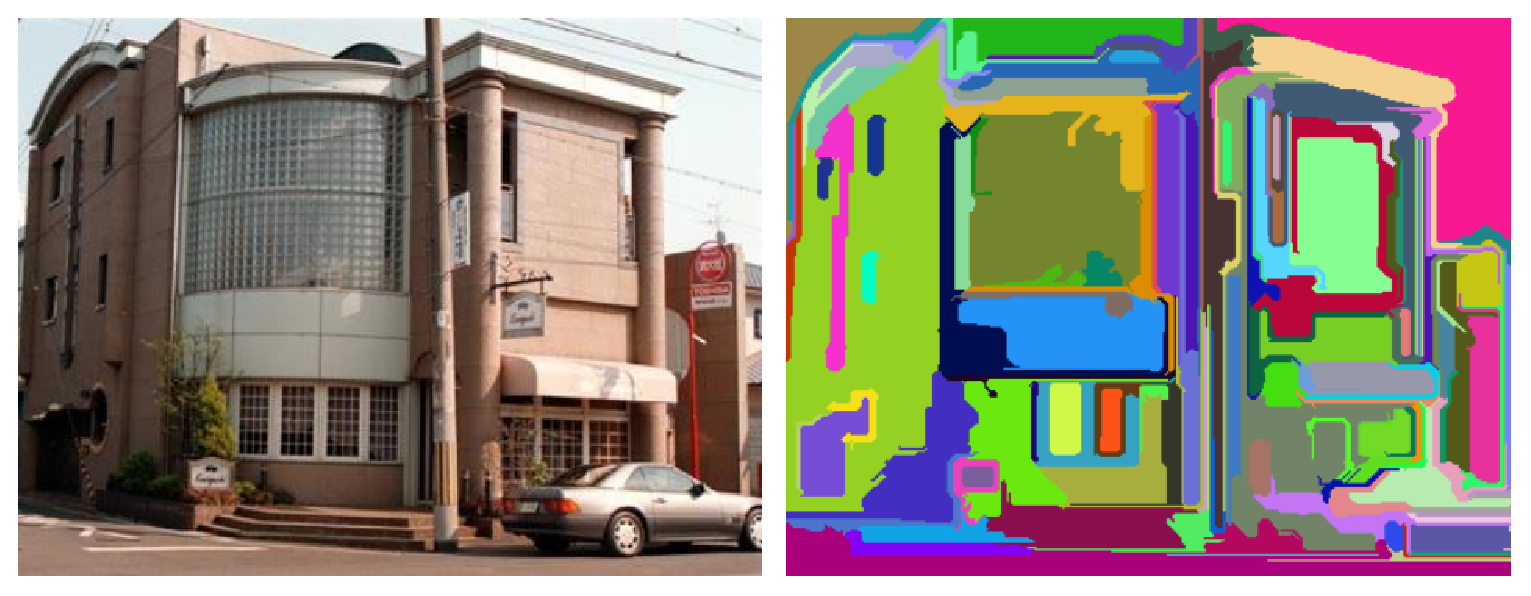
\includegraphics[keepaspectratio=true, width=\linewidth]{segment.eps}
  \caption{A monocular image with the over-segmentation produced by
           Felzenszwalb et al. ~\cite{Felzen}. These segmenst are refered to as
           super pixels.}
  \label{fig:superpixel}
\end{figure}

We propose a system that combines these two efforts. It attempts to reconstruct
the scene geometry from a monocular video instead of a monocular image. This
allows the system to incorporate temporal information into the surface
estimations. However, structure from motion or similar techniques cannot be
applied to the video since there is no information about the camera or defined
camera locations. As a result, the system relies upon the methods developed by
Hoiem et al. ~\cite{Hoiem-05} and Sexana et al. ~\cite{Sexana} to find the
vertical surface orientations. From this the relative depth of different
regions of the image can be estimated to provide object information. The goal
is to create a depth segmentation of the image.

The system uses supervised learning to create a classifier for image regions.
The system will start with an over-segmentation of the image to produce super
pixels. Super pixels are simply image regions that statistical information can
gathered for. The statistical information is used as input for the learned
classifier which is used to decide the surface orientations. From the surface
orientations we can gather depth information by simply using where the vertical
surfaces intersect the horizontal surface defined by the ground plane.

%-------------------------------------------------------------------------
\Section{Super Pixels}

\begin{figure*}[t]
  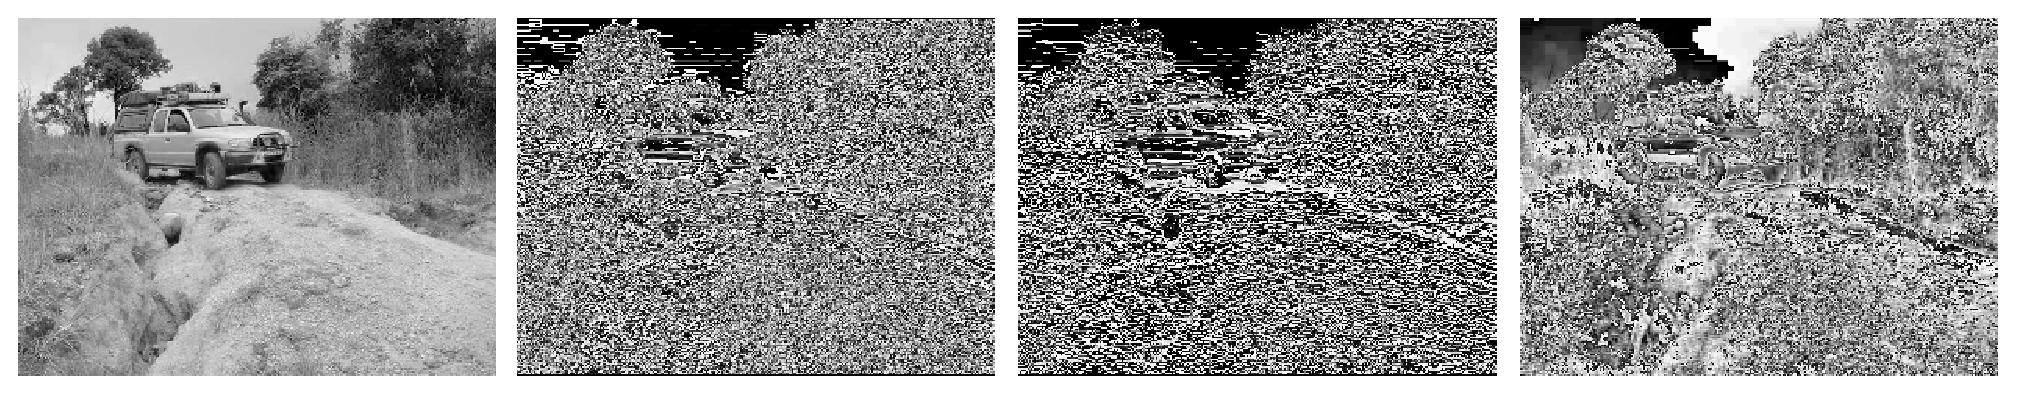
\includegraphics[keepaspectratio=true, width=\textwidth]{Laws.eps}
  \caption{One color channel of a source image with the Law's mask
           convolutions. The average response from these masks is used
           as one of the features for the classifier.}
  \label{fig:lawsconv}
\end{figure*}

The first step in finding a usable depth segmenation is to perform an
over-segmentation of the image. An example of the over-segmenation can be seen
in Figure ~\ref{fig:superpixel}. These super pixels will be used as the units
of surface. We will construct the surfaces out of the individual super pixels
and the borders between surfaces will be assumed to fall on the boundaries
between super pixel. As a result of this, the only requirement of the
over-segmentaion is that there is no single super pixel that spans two real
world surfaces within the image. If a superpixel does fall on two different
real world surfaces, then it would have multiple orientation and automatically
cause the depth segmentation to be invalid. The system uses the segmenation
algorithm described by Felzenszwalb et al. ~\cite{Felzen} to produce the super
pixel image. Any segmenation algorithm could be used in instead as long as it
doesn't produces any segments that contain two distinct real world surfaces.

For each super pixel in the image a set of statistics are calculated. The major
distinguishing factors between horizontal and vertical surfaces are the
textures and line orientations on the surface. As a result, the texture is
calculated as the response the a set of 3x3 Law's masks for the different color
channels of the image. The Law's masks are created using the three vectors
[1, 2, 1], [1, 0, -1], and [1, -1, 1]. These vectors are multiplied to get
9 3x3 masks that are convolved with the color channel. This produces a total of
27 responses from the Law's masks. A source image and some example responses
for the Law's masks can be seen in Figure ~\ref{fig:lawsconv}. A histogram of
gradient orientations is calculated for each super pixel as well. 18 buckets
are used for the histogram of gradients, and each color channel uses a
different histogram. This gives a total of 54 buckets from gradient histograms.
This gives an 81 dimensional space that is used to represent the super pixel in
the learned classifier.

%-------------------------------------------------------------------------
\Section{Learned Classifier}

\begin{figure*}[t]
  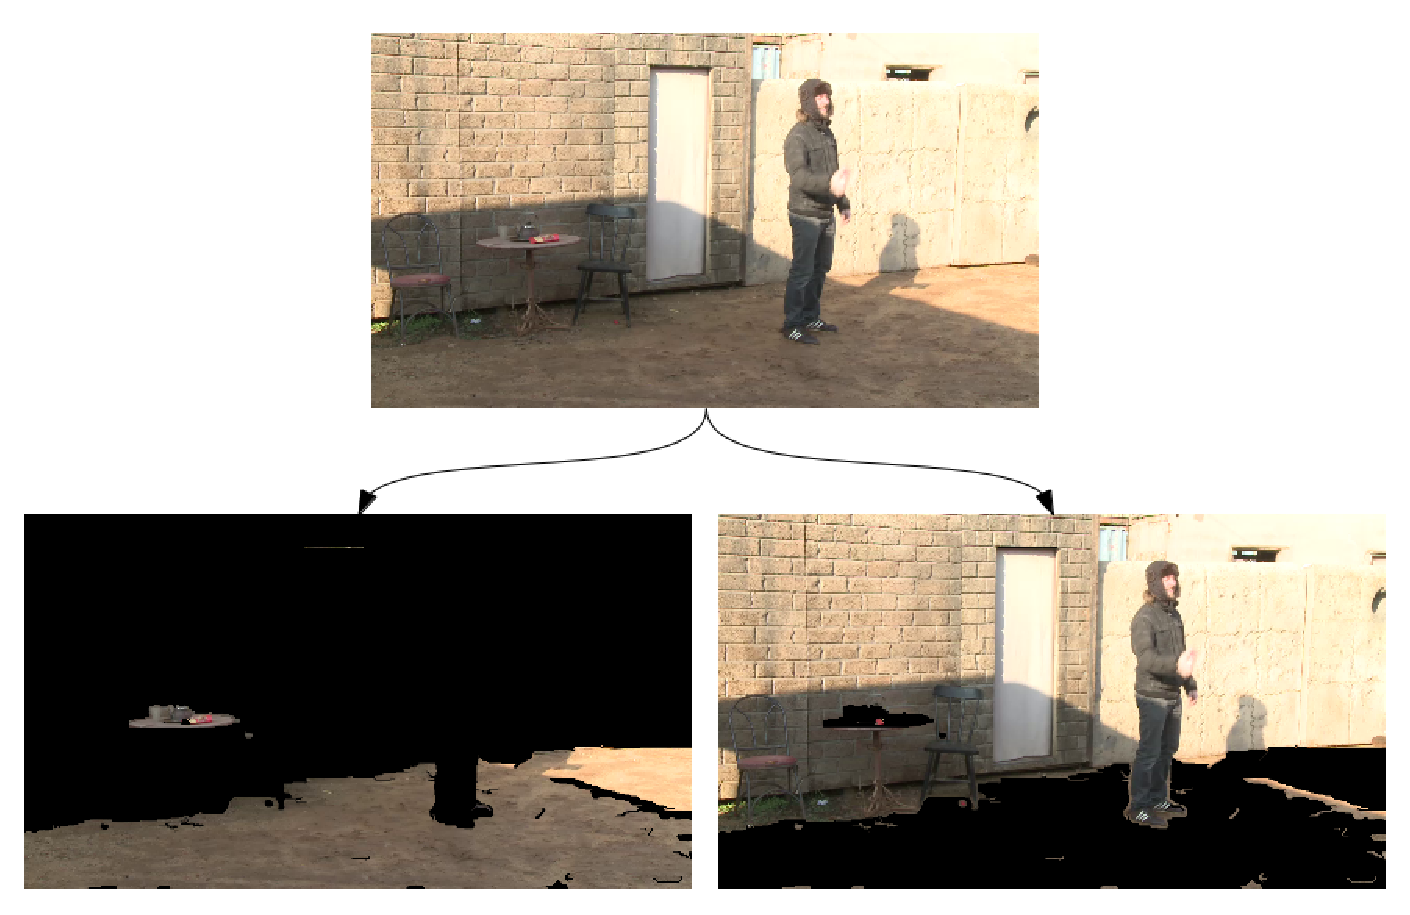
\includegraphics[keepaspectratio=true, width=\textwidth]{split.eps}
  \caption{The output of the classifier. Image regions of the source image
           (the top image) are input into the classiefier. The super pixels
           that the classifier decided were horizontal are on the left. The
           vertical are on the right. }
  \label{fig:spliting}
\end{figure*}

The collection of features used for each super pixel is fed into a learning
classifier that will inform the system about the orienations of the super
pixels. Both grouping the super pixels togther into larger image regions and
testing super pixels completely independently was tried. Two different learned
classifiers were used. The discrete form of Adaboost and a simple k-nearest
classifires were both tested and the results compared. These were used becuase
of the simplicity involved in using them correctly.

Both individual super pixels and small image regions were used as input for the
classifier. These were tested individually for the training and testing phases.
The rational behind testing image region is that the orientation can be
informed by what lies around the super pixel. For example, take the case of a
brick wall where the boundaries between the super pixels would fall at the edge
of each brick. If we include adjacent super pixels in the calculation of the
score for the relevant super pixel, then we can include more of the texture of
the brick wall. We are pulling more information into the surface estimations in
the hopes that we will get a better response.

Once an image has been over-segmented, each super pixel is used as input into
the classifier. The results of the classifier are then used to directly label
the image as either vertical or horizontal. The image is split into these two
seperate segments as in Figure ~\ref{fig:spliting}.

%-------------------------------------------------------------------------
\Section{Results}

\begin{figure*}[t]
  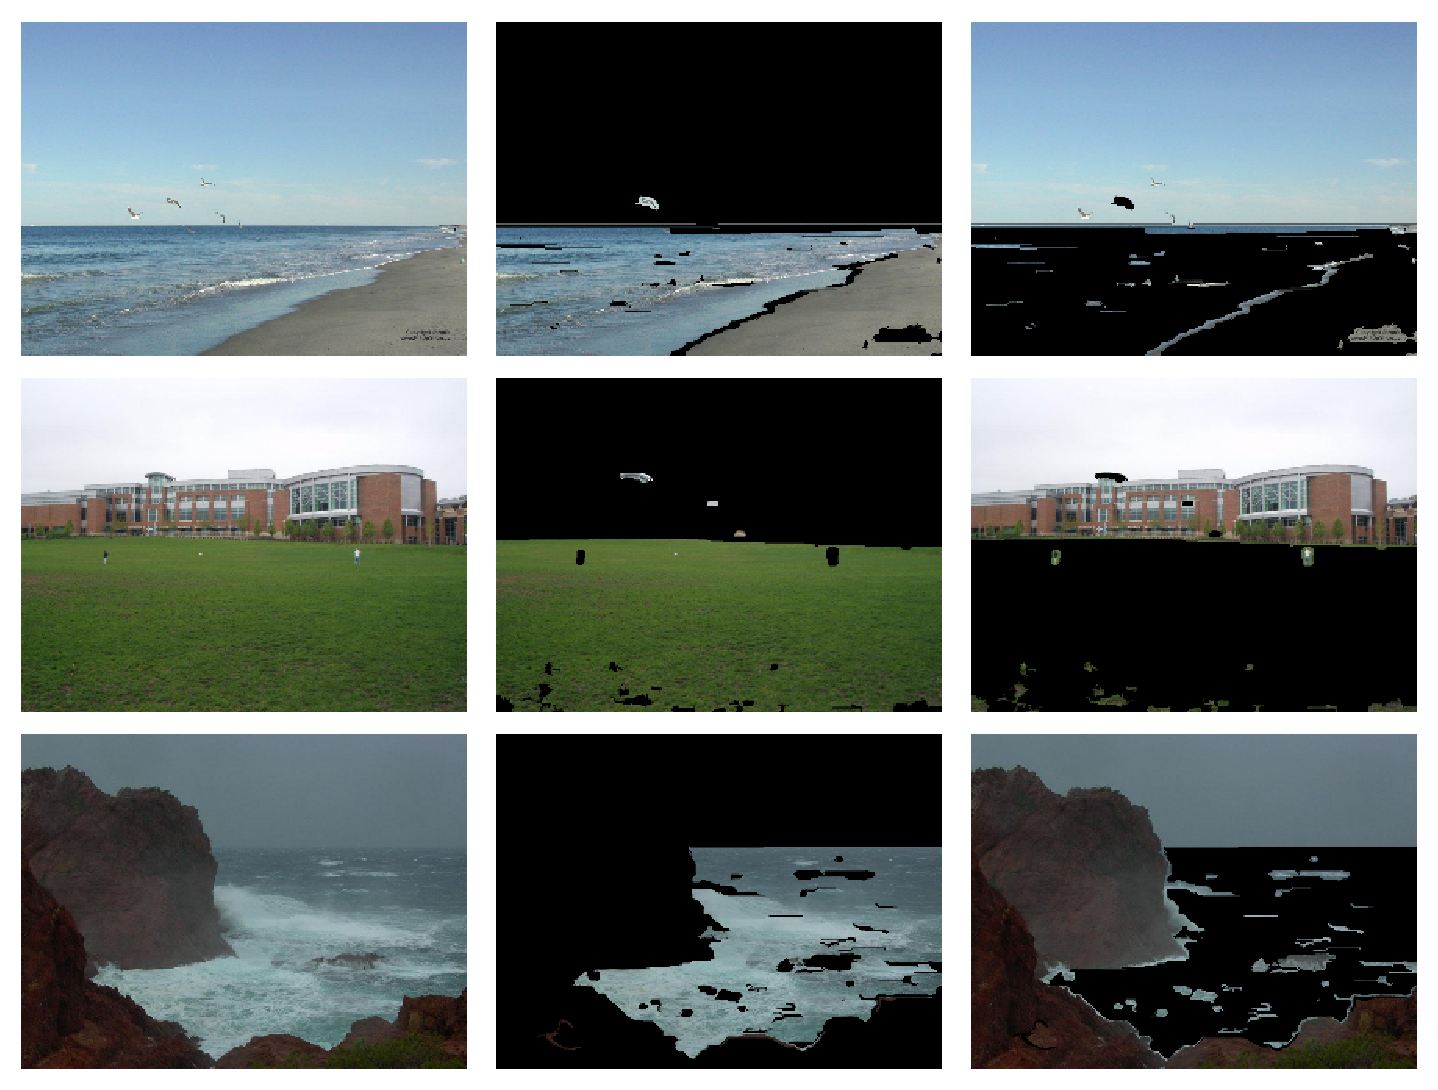
\includegraphics[keepaspectratio=true, width=\textwidth]{Good.eps}
  \caption{ Examples or correct segmented images. The first column is the
            original source image. The middle column is the horizontal segment
            of the image. The right column is the vertical segment of the image}
  \label{fig:correct}
\end{figure*}


%-------------------------------------------------------------------------
\bibliographystyle{depth}
\bibliography{depth}

\end{document}

